% Tikz File 'architecture_pregel.tex'
\documentclass{standalone}
\usepackage{tikz}
\usetikzlibrary{positioning,fit}
\begin{document}
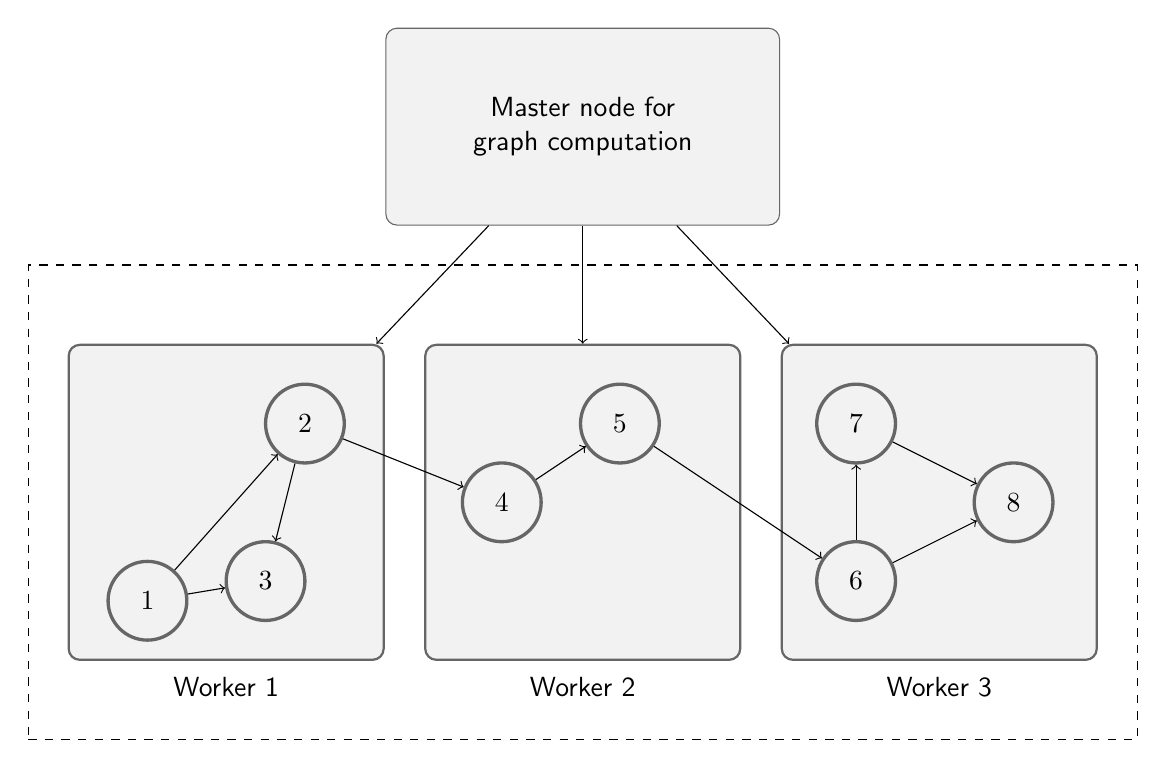
\begin{tikzpicture}[
        master/.style={rectangle, rounded corners, draw=black!60, fill=black!5, text centered, minimum width=50mm, minimum height=25mm, text width=40mm},
        worker/.style={rectangle, rounded corners, draw=black!60, fill=black!5, thick, minimum size=40mm},
        vertex/.style={circle, draw=black!60, fill=black!5, very thick, minimum size=10mm},
    ]
    \node[worker,label={[yshift=-4.6cm, font=\sffamily]Worker 1}] (worker1) {};
    \node[worker,label={[yshift=-4.6cm, font=\sffamily]Worker 2}] (worker2) [right=0.5cm of worker1] {};
    \node[worker,label={[yshift=-4.6cm, font=\sffamily]Worker 3}] (worker3) [right=0.5cm of worker2] {};
    \node[master,font=\sffamily] (master) [above=1.5cm of worker2] {Master node for graph computation};

    \node[vertex] (V1) at (-1, -1.25) {1};
    \node[vertex] (V2) at (1, 1) {2};
    \node[vertex] (V3) at (0.5, -1) {3};
    \node[vertex] (V4) at (3.5, 0) {4};
    \node[vertex] (V5) at (5, 1) {5};
    \node[vertex] (V6) at (8, -1) {6};
    \node[vertex] (V7) at (8, 1) {7};
    \node[vertex] (V8) at (10, 0) {8};

    \node[fit={(worker1)(worker2)(worker3)},draw,dashed,inner xsep=5mm,inner ysep=10mm] (workers) {};

    \path[-to] (V1) edge node {} (V2);
    \path[-to] (V2) edge node {} (V3);
    \path[-to] (V1) edge node {} (V3);

    \path[-to] (V2) edge node {} (V4);
    \path[-to] (V4) edge node {} (V5);
    \path[-to] (V5) edge node {} (V6);

    \path[-to] (V6) edge node {} (V7);
    \path[-to] (V6) edge node {} (V8);
    \path[-to] (V7) edge node {} (V8);

    \path[-to] (master) edge node {} (worker1);
    \path[-to] (master) edge node {} (worker2);
    \path[-to] (master) edge node {} (worker3);
\end{tikzpicture}
\end{document}